\documentclass[UTF8]{ctexart}
\usepackage{amsmath}
\usepackage{geometry}
\usepackage{graphicx}
\usepackage{gensymb}
\usepackage{titlesec}
\usepackage{wrapfig}
\usepackage{float}
\geometry{a4paper,scale=0.8}
\title{2018年电磁场与波期末试题}
\author{Deschain}
\titlespacing*{\section}
{0pt}{0pt}{0pt}
\begin{document}
\titlespacing*{\subsection}
{0pt}{0pt}{0pt}
\titlespacing*{\paragraph}
{0pt}{0pt}{0pt}
\titlespacing*{\subparagraph}
{0pt}{0pt}{0pt}
\maketitle
\section{}
\begin{wrapfigure}{r}{4cm}
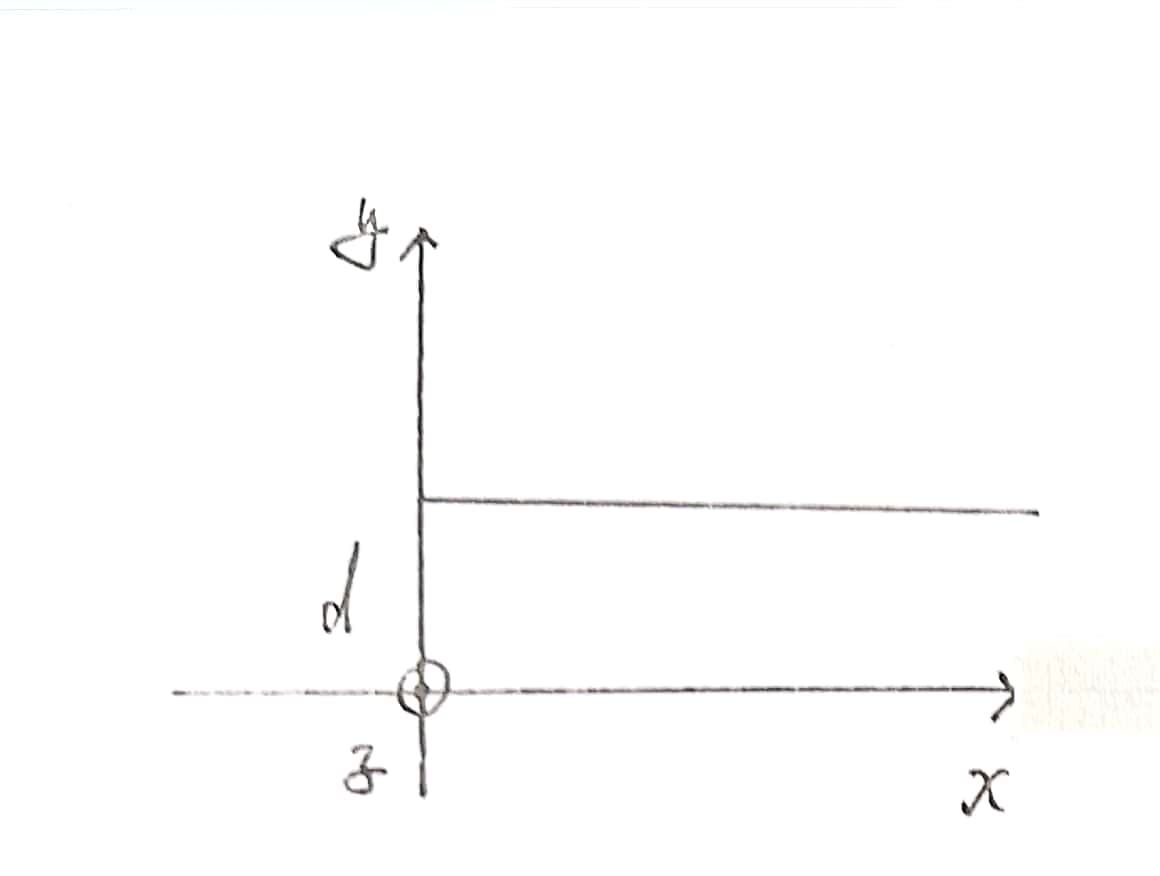
\includegraphics[width=4cm]{2018-1.jpg}
\end{wrapfigure}
\paragraph{}
两无限大磁壁,300MHz的电磁场沿x轴正向传播。
\subsection{}
\paragraph{}
d=5mm时,可以传播电磁波吗?如果可以,画出$[0,\lambda_x]$的三维电磁场结构;如果不可以,请说明理由。
\subparagraph{解答}
可以传播TEM波。
\begin{figure}[htbp]
\centering
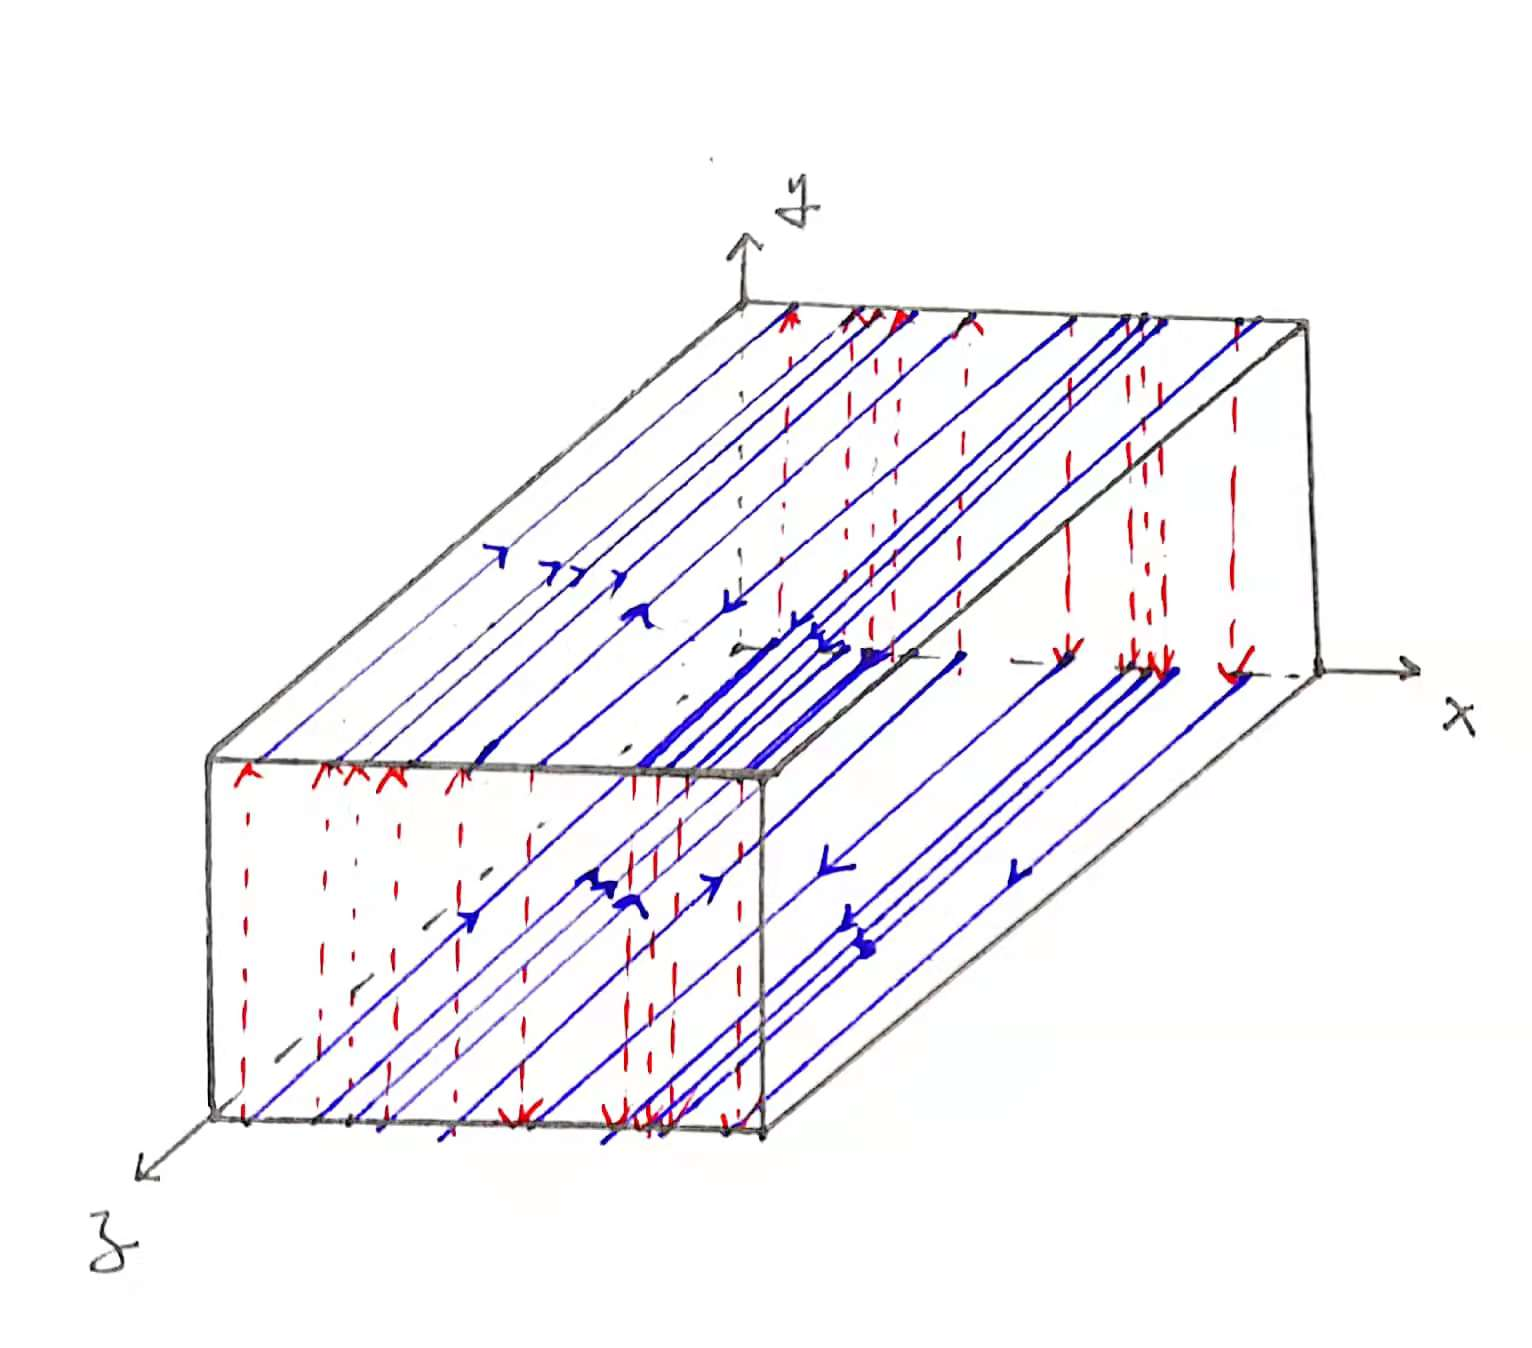
\includegraphics[width=6cm,height=3cm]{2018-2.jpg}
\end{figure}
\subsection{}
\paragraph{}
若要传播300MHz的TE波,d的最小尺寸是多少?
\subparagraph{}
\begin{equation*}
d \geq \frac{\pi}{k}=0.5m
\end{equation*}
\subsection{}
\paragraph{}
写出TE基模的复数表达式(包含波动项,时谐项)。
\subparagraph{解答}
\begin{equation*}
\begin{aligned}
&\vec E=\hat zjsin(\frac{n\pi}{d}y)e^{j(\omega t-kx)}\\
&\vec H=(\hat xcos(\frac{n\pi}{d}y)+\hat yjsin(\frac{n\pi}{d}y))e^{j(\omega t-kx)}
\end{aligned}
\end{equation*}
\subsection{}
\paragraph{}
画出$[0,\lambda_x]$的TE基模三维电磁场结构(电场用实线,磁场用虚线)。
\begin{figure}[htbp]
\centering
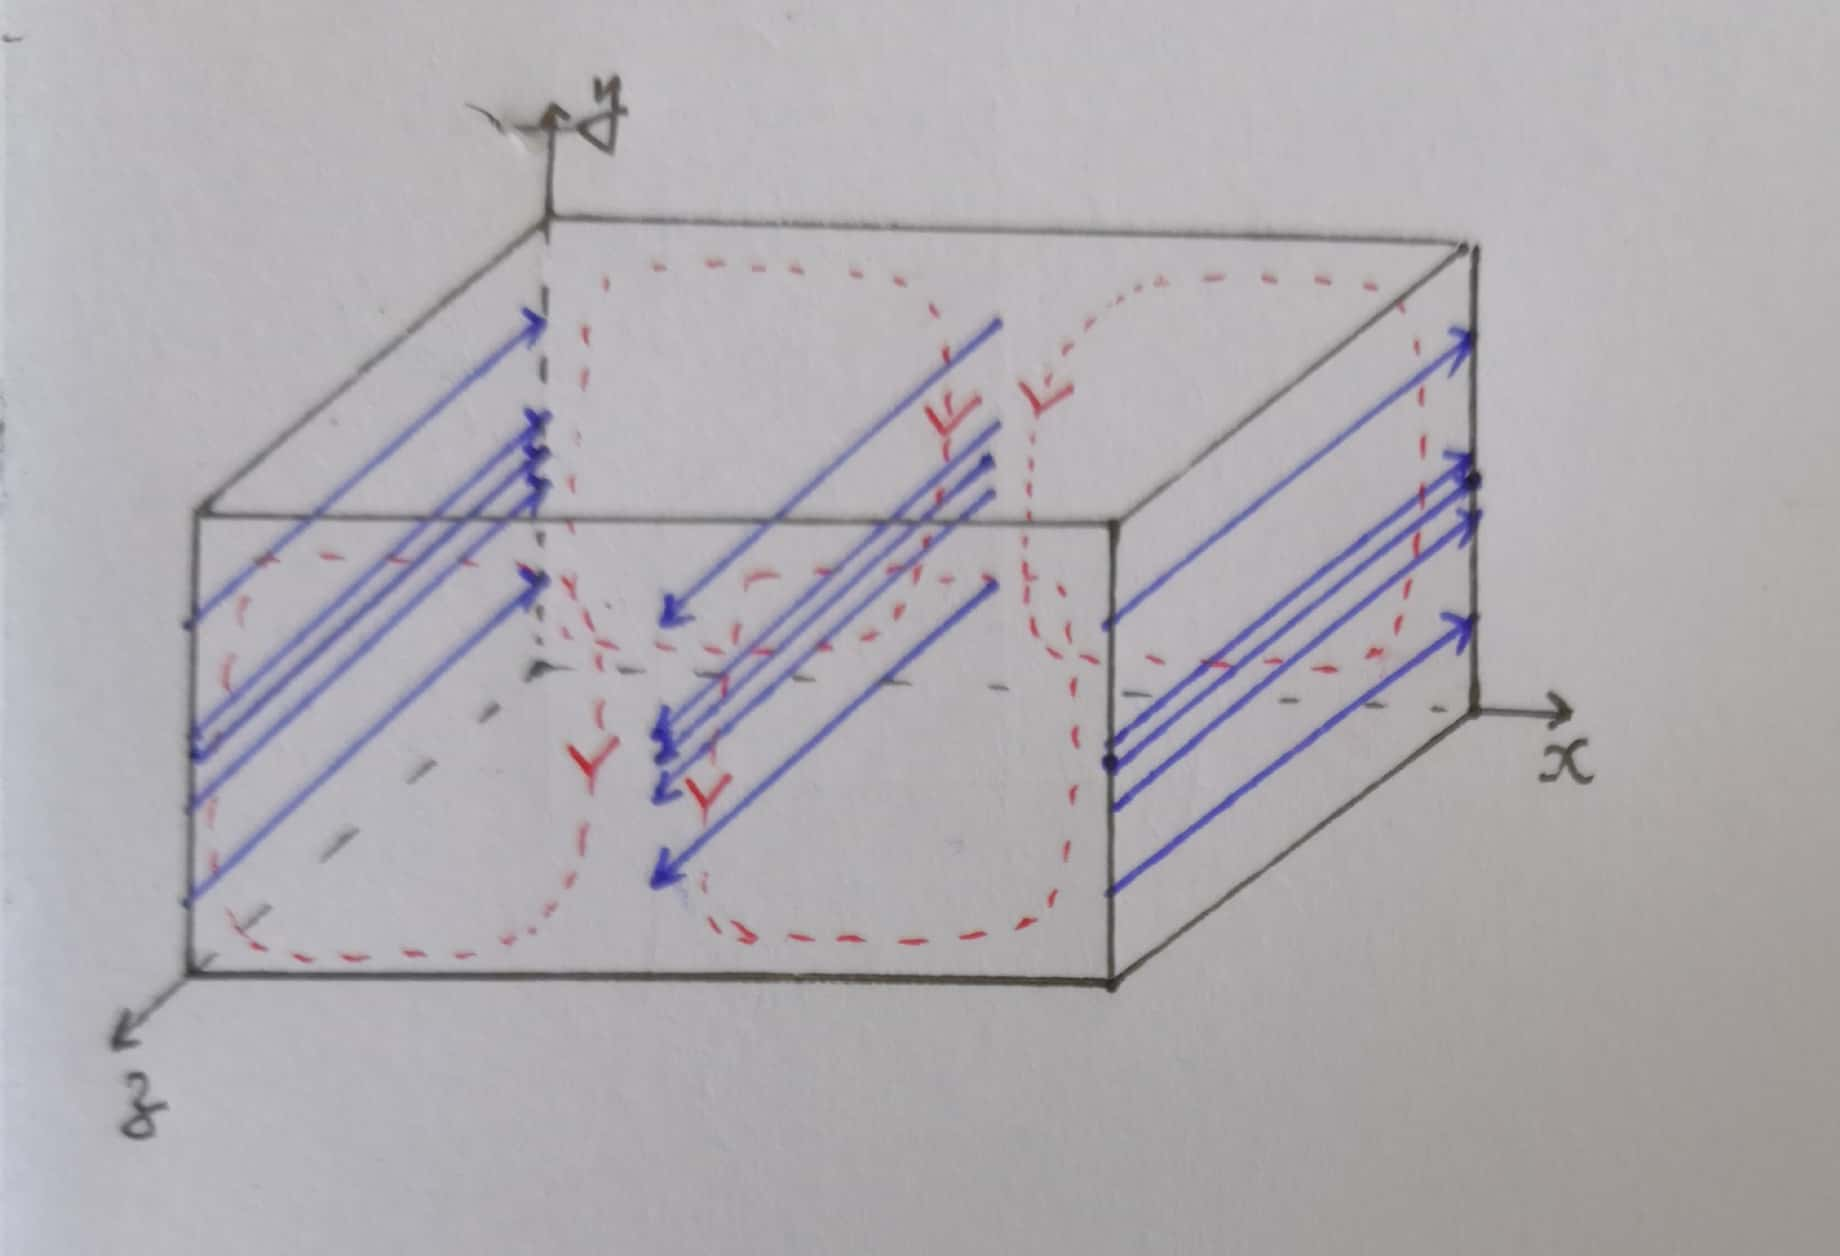
\includegraphics[width=6cm,height=3cm]{2018-3.jpg}
\end{figure}
\subsection{}
\paragraph{}
画出$[0,\lambda_x]$的TM基模三维电磁场结构(电场用实线,磁场用虚线)。
\begin{figure}[htbp]
\centering
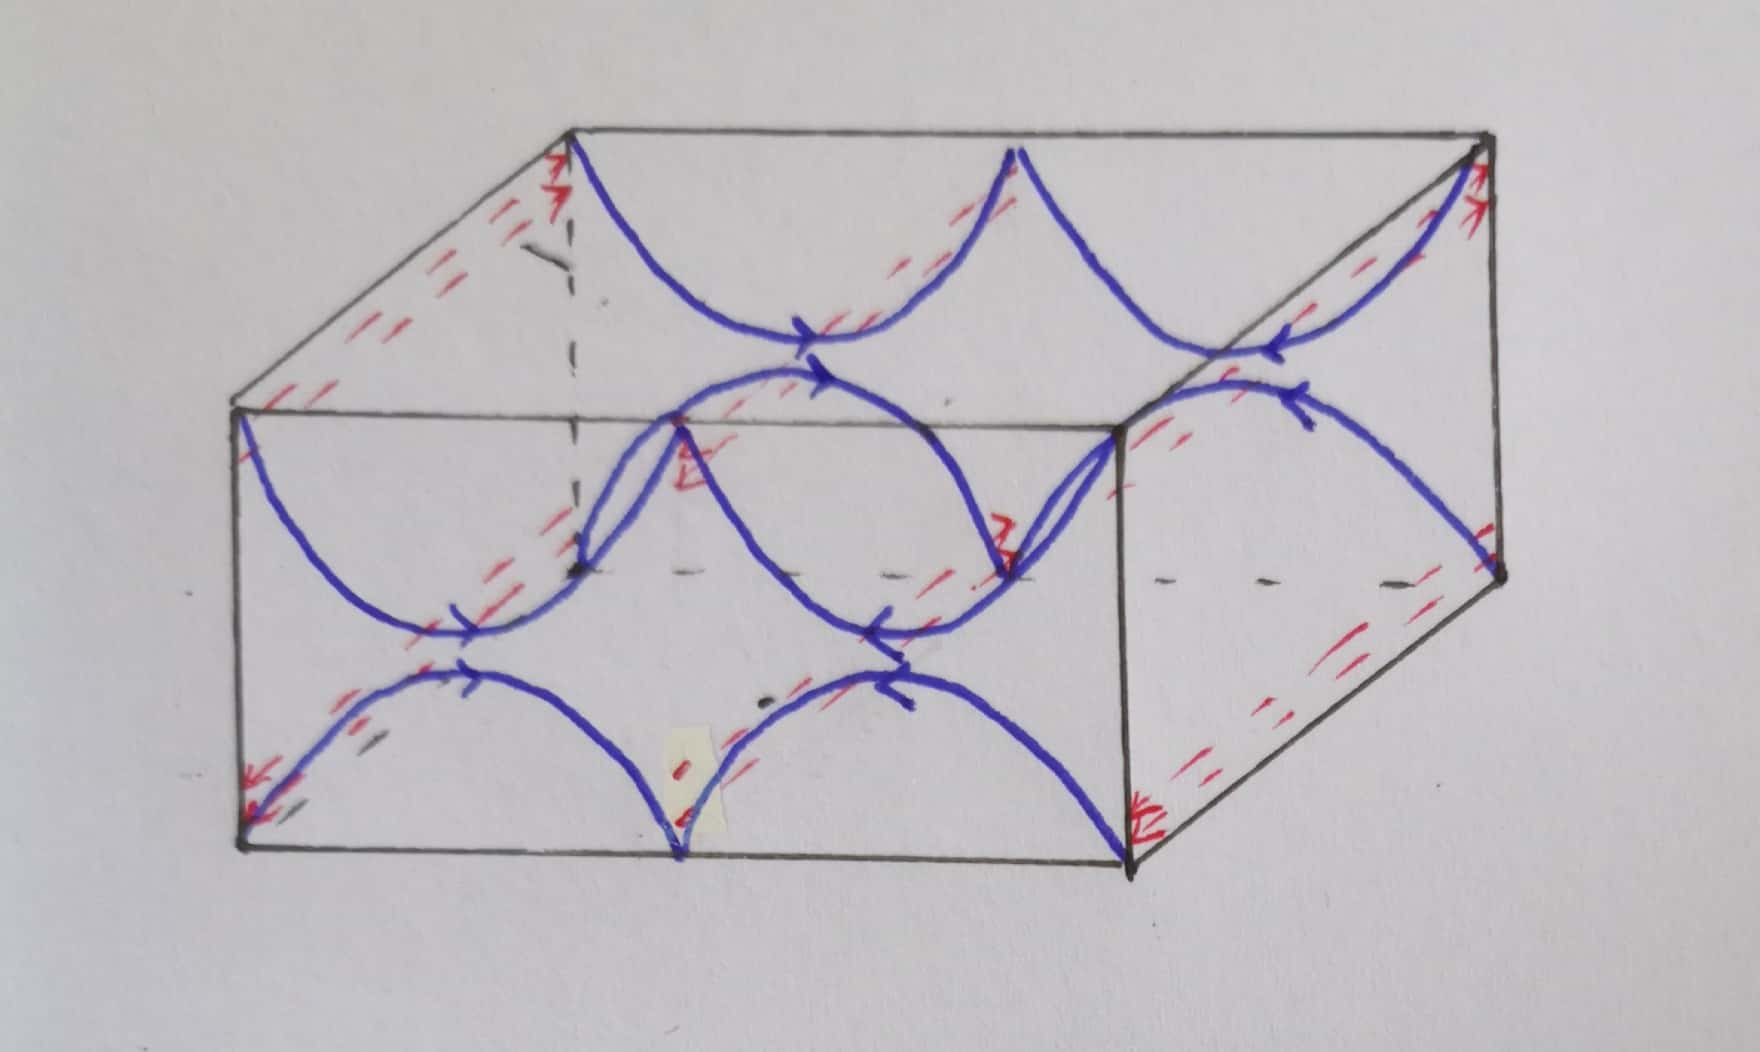
\includegraphics[width=6cm,height=3cm]{2018-4.jpg}
\end{figure}
\section{}
\subsection{}
\paragraph{静电场}
在Z轴远离原点处产生方向为$\frac{\sqrt 3}{3}\hat x+\frac{\sqrt 3}{3}\hat y+\frac{\sqrt 3}{3}\hat z$的磁场。写出磁偶极子方向、相对大小。
\subparagraph{}
沿x轴正向:沿y轴正向:沿z轴正向=2:2:1
\subsection{}
\paragraph{时变电磁场}
是否能在Z轴远离原点处产生方向为$\frac{\sqrt 3}{3}\hat x+\frac{\sqrt 3}{3}\hat y+\frac{\sqrt 3}{3}\hat z$的磁场分量?为什么?
\subparagraph{解答}
不能。辐射场没有$\hat r$分量。
\subsection{}
\paragraph{}
在$\pm y$轴、$\pm z$轴远处产生左旋圆极化波,需要在原点附近怎样放置磁偶极子?
\subparagraph{解答}
沿x轴正向放置电偶极子和磁偶极子,两者在y轴同一位置产生的电场等大,且电偶极子的电场超前磁偶极子的电场$\frac{\pi}{2}$。
\subsection{}
\paragraph{}
写出Z轴负向远处的左旋圆极化波表达式。
\subparagraph{解答}
\[\vec E=E_0(\hat x-j\hat y)e^{j(\omega t+kz)}\]
\section{}
\paragraph{}
如右图,长宽高为$20\times 20\times 30$,五面均为5V。Z=0平面Y>0时$\varphi=10V$,Z=0平面Y<0时$\varphi=0V$。
\subparagraph{解答}
$\varphi_1$相当于:“Z=0平面上,Y>0时$\varphi=5V$,Y<0时$\varphi=-5V$”。
\begin{equation*}
\begin{aligned}
&\varphi_1(x,y,z)=\sum_{n}^{}\sum_{m}^{}A_{mn}sin(\frac{n\pi}{a}x)sin(\frac{m\pi}{b}y)sh(\sqrt{{\frac{n\pi}{a}}^2+{\frac{m\pi}{b}}^2}(c-z))\\
&n=1,3,5,\cdots \quad\quad m=2,4,6,\cdots\\
\varphi=\varphi_1+5
\end{aligned}
\end{equation*}
\subsection{}
\paragraph{}
求区域内电势$\varphi(\vec r)$。
\paragraph{}
画出X=10的平面电力线(实线)和电位线(虚线)。
\begin{figure}[H]
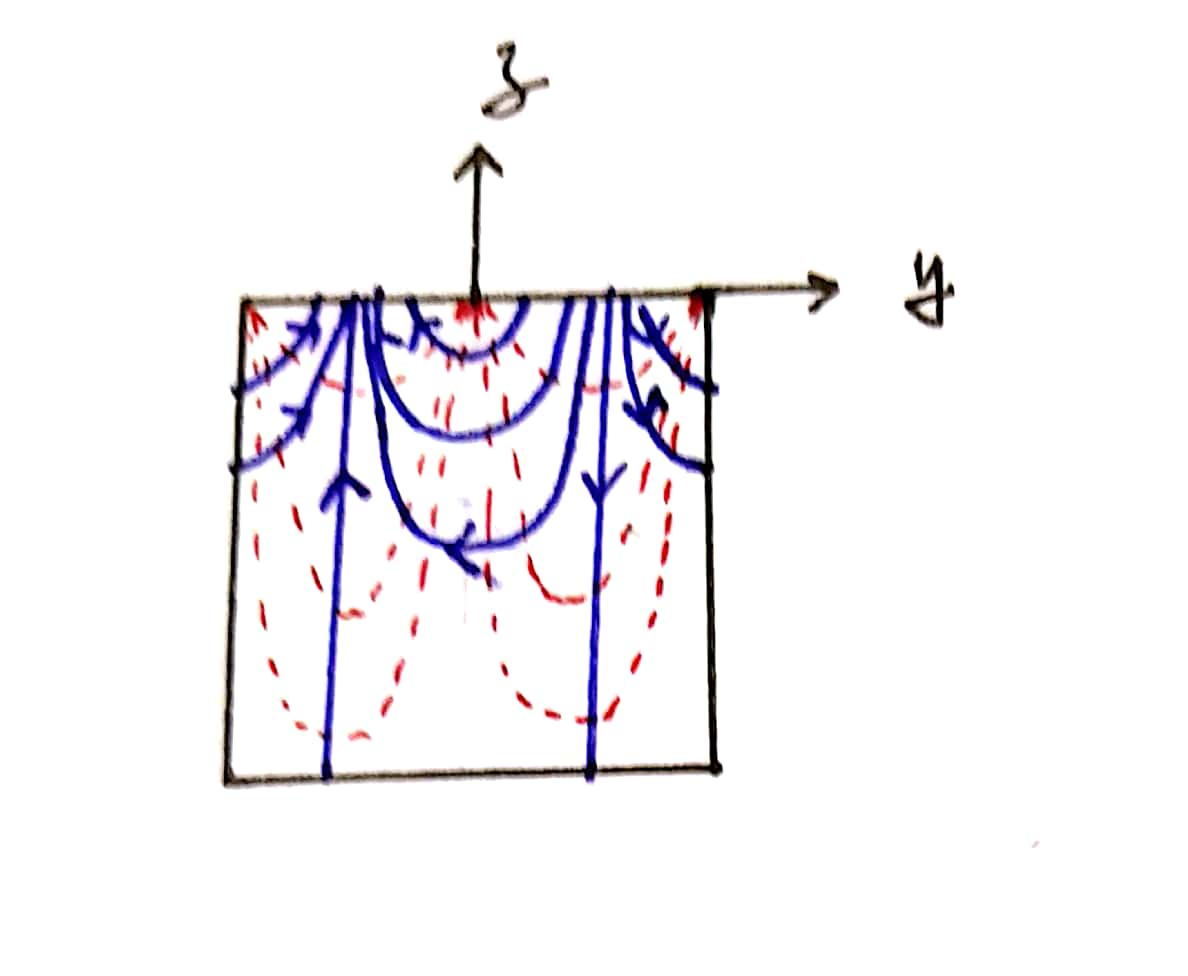
\includegraphics[width=3cm,height=2cm]{2018-5.jpg}
\centering
\end{figure}
\section{}
右图是一个二维静电场。
\begin{figure}[htbp]
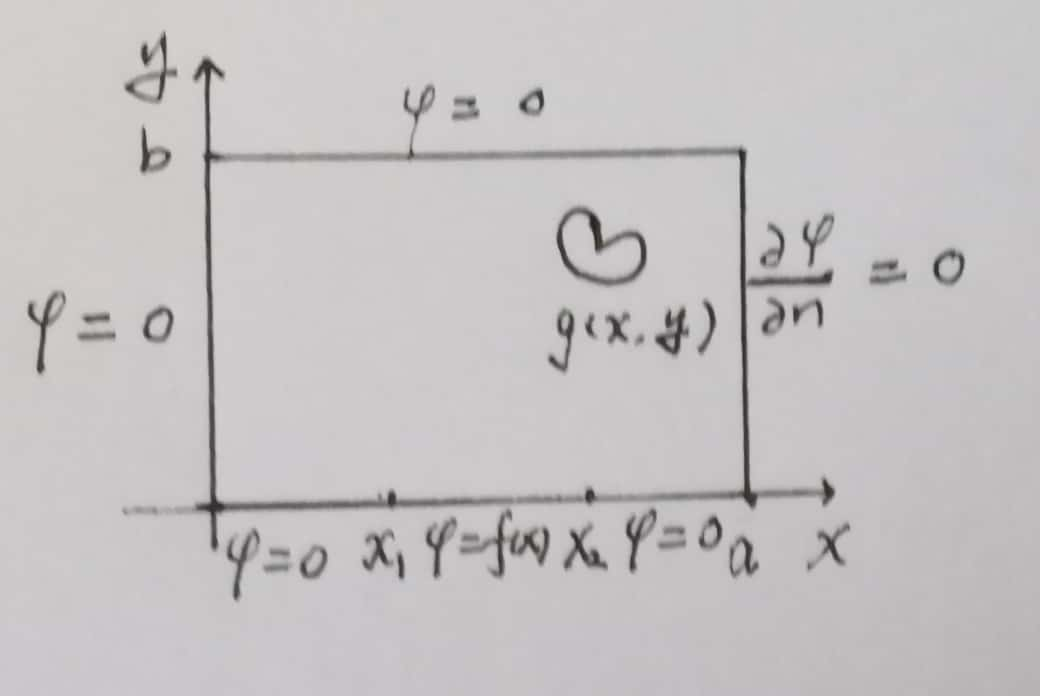
\includegraphics[width=6cm,height=4cm]{2018-6.jpg}
\centering
\end{figure}
\subsection{}
\paragraph{}
求格林函数G满足的偏微分方程。
\subparagraph{解答}
\[\nabla^2G(\vec r,\vec r')=-\delta(\vec r,\vec r')\]
\subsection{}
\paragraph{}
求G满足的边界条件。
\subparagraph{解答}
将原区域以$x=a$为轴做对称。
\[G\lvert_{y=b}=0, G\lvert_{y=0}=0, G\lvert_{x=2a}=0, G\lvert_{x=0}=0\]
\subsection{}
\paragraph{}
求G的解析式。
\subparagraph{解答}
$0<y<y'$为1区,$y'<y<b$为2区。
\begin{figure}[htbp]
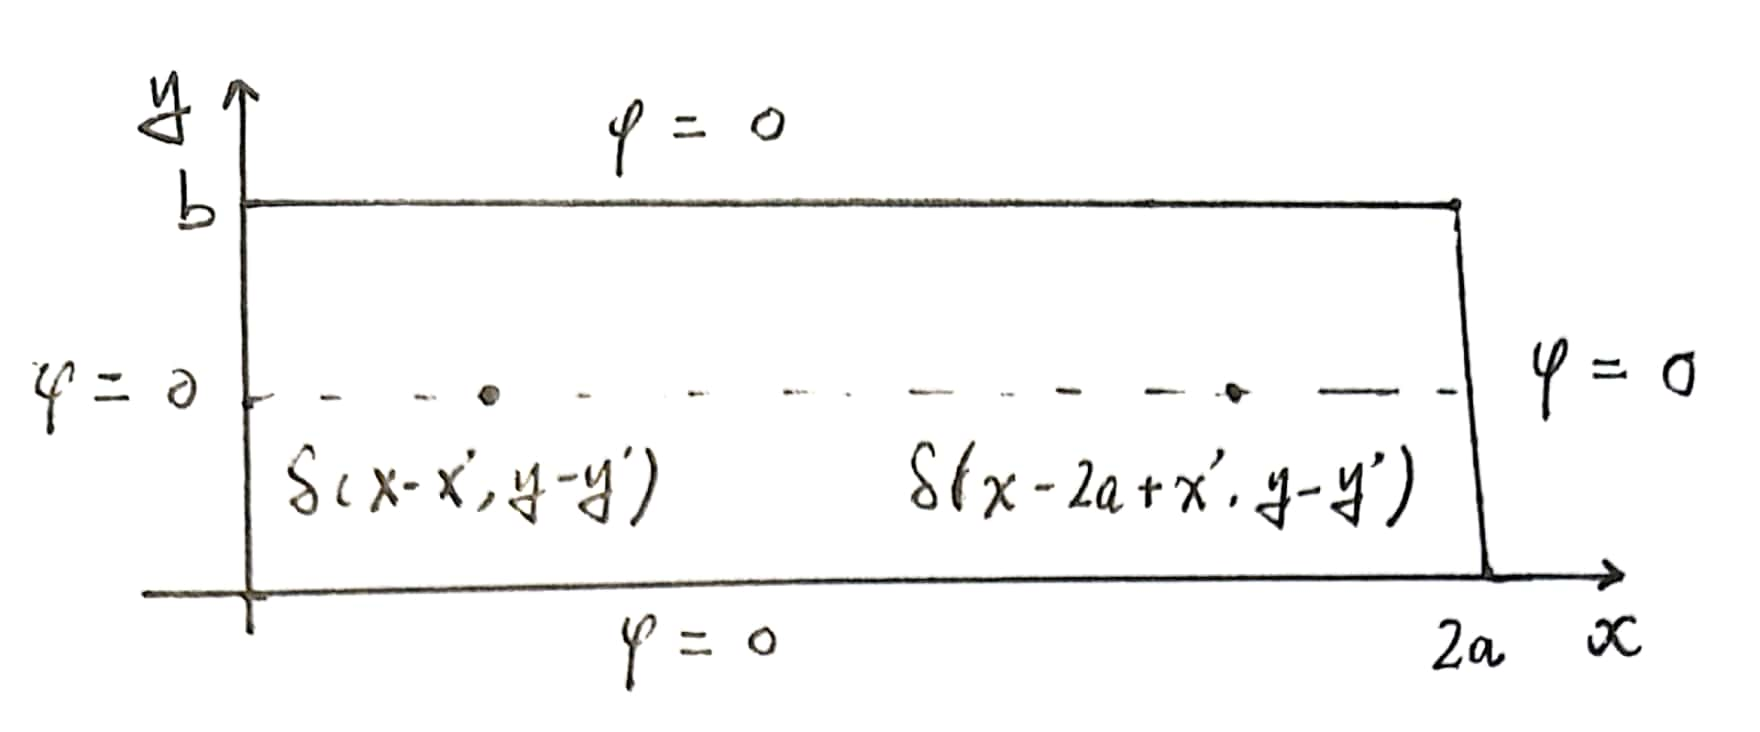
\includegraphics[width=10cm,height=4cm]{2018-7.jpg}
\centering
\end{figure}
\begin{equation*}
\begin{aligned}
&G^1(x,x',y,y')=sum_n^{\infty}A_nsin(\frac{n\pi}{2a}x)sh(\frac{n\pi}{2a}y),n=1,3,5\cdots\\
&G_2(x,x',y,y')=sum_m^{\infty}B_msin(\frac{m\pi}{2a}x)sh(\frac{m\pi}{2a}(b-y)),m=1,3,5\cdots\\
&\frac{\partial G_1}{\partial y}-\frac{\partial G_2}{\partial y}\lvert_{y=y'}=\delta(x-x')+\delta(x-2a+x')\\
&G_1-G_2\lvert_{y=y'}=0
\end{aligned}
\end{equation*}
\subsection{}
\paragraph{}
写出化简后$\varphi$的表达式。
\subparagraph{解答}
\[\varphi(\vec r)=\int_S^{}{\frac{\rho G}{\varepsilon}dS}-\int_{x_1}^{x_2}{f(x)Gdx}\]
其中S是g(x,y)存在的区域。
\subsection{}
\paragraph{}
格林函数点电荷在(x',y')处时,画出区域内的电力线(实线)和电位线(虚线)。
\begin{figure}[htbp]
\centering
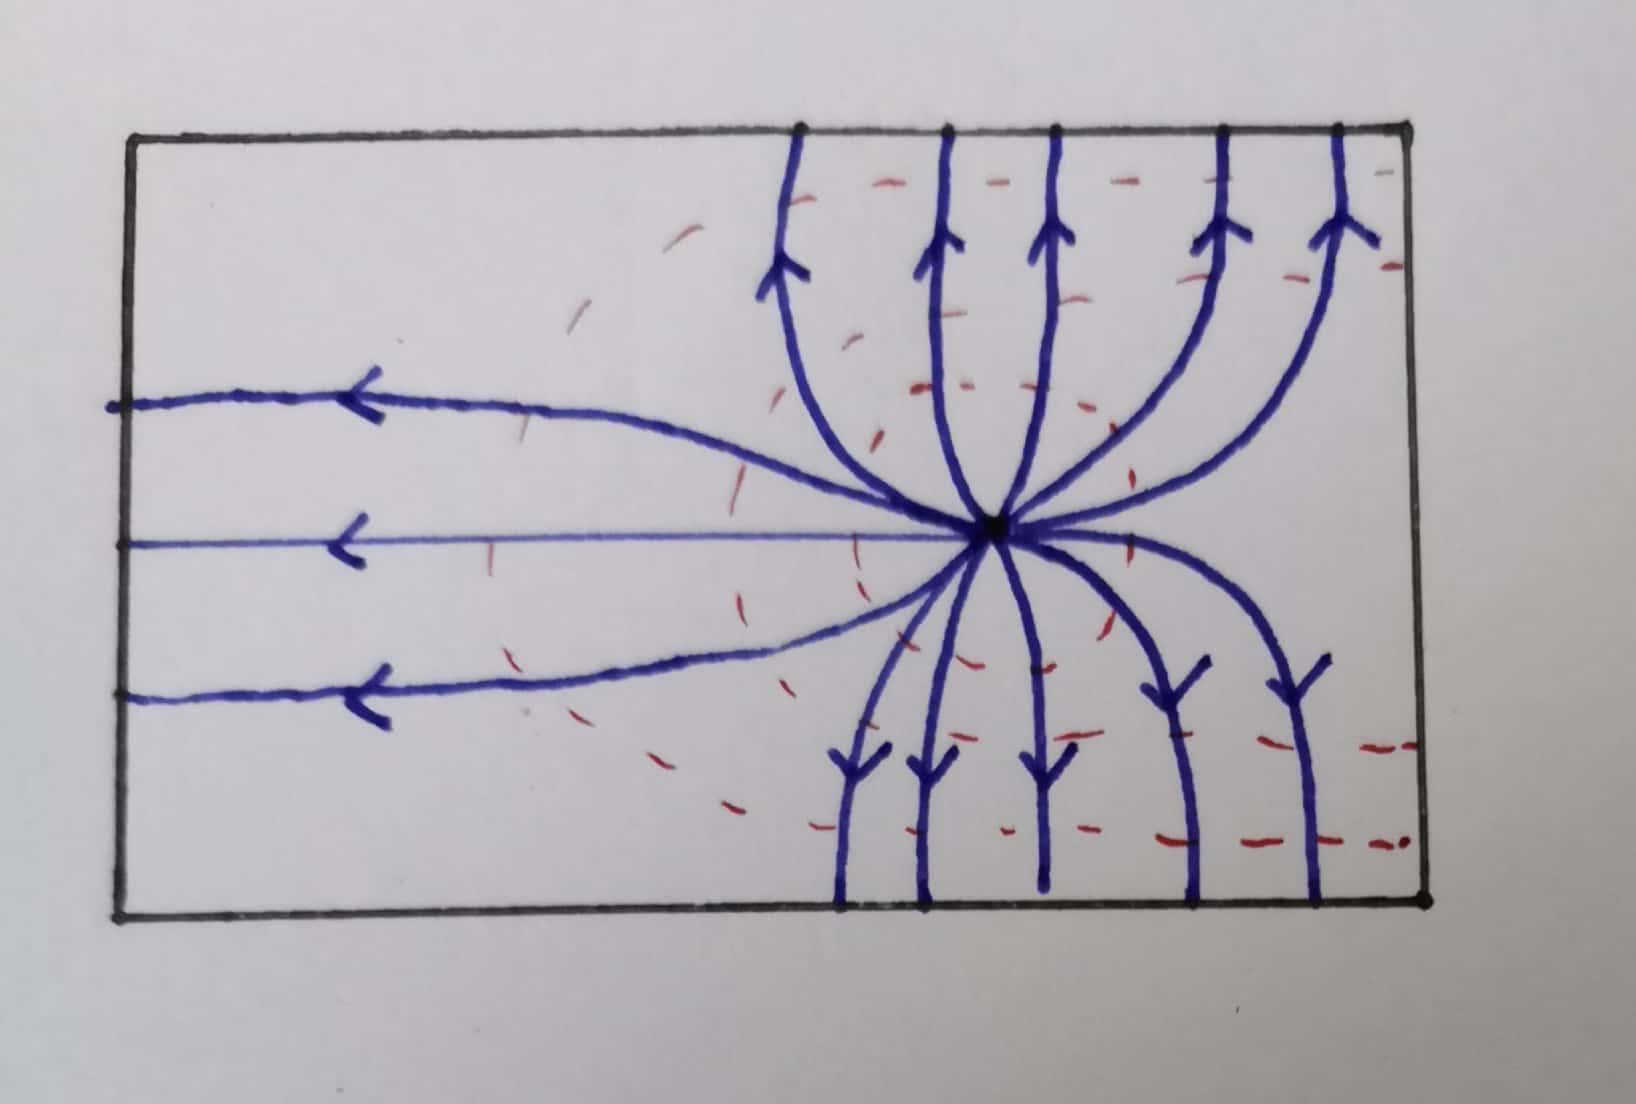
\includegraphics[width=6cm,height=4cm]{2018-8.jpg}
\end{figure}
\end{document}